\documentclass{article}\usepackage[]{graphicx}\usepackage[]{xcolor}
% maxwidth is the original width if it is less than linewidth
% otherwise use linewidth (to make sure the graphics do not exceed the margin)
\makeatletter
\def\maxwidth{ %
  \ifdim\Gin@nat@width>\linewidth
    \linewidth
  \else
    \Gin@nat@width
  \fi
}
\makeatother

\definecolor{fgcolor}{rgb}{0.345, 0.345, 0.345}
\newcommand{\hlnum}[1]{\textcolor[rgb]{0.686,0.059,0.569}{#1}}%
\newcommand{\hlsng}[1]{\textcolor[rgb]{0.192,0.494,0.8}{#1}}%
\newcommand{\hlcom}[1]{\textcolor[rgb]{0.678,0.584,0.686}{\textit{#1}}}%
\newcommand{\hlopt}[1]{\textcolor[rgb]{0,0,0}{#1}}%
\newcommand{\hldef}[1]{\textcolor[rgb]{0.345,0.345,0.345}{#1}}%
\newcommand{\hlkwa}[1]{\textcolor[rgb]{0.161,0.373,0.58}{\textbf{#1}}}%
\newcommand{\hlkwb}[1]{\textcolor[rgb]{0.69,0.353,0.396}{#1}}%
\newcommand{\hlkwc}[1]{\textcolor[rgb]{0.333,0.667,0.333}{#1}}%
\newcommand{\hlkwd}[1]{\textcolor[rgb]{0.737,0.353,0.396}{\textbf{#1}}}%
\let\hlipl\hlkwb

\usepackage{framed}
\makeatletter
\newenvironment{kframe}{%
 \def\at@end@of@kframe{}%
 \ifinner\ifhmode%
  \def\at@end@of@kframe{\end{minipage}}%
  \begin{minipage}{\columnwidth}%
 \fi\fi%
 \def\FrameCommand##1{\hskip\@totalleftmargin \hskip-\fboxsep
 \colorbox{shadecolor}{##1}\hskip-\fboxsep
     % There is no \\@totalrightmargin, so:
     \hskip-\linewidth \hskip-\@totalleftmargin \hskip\columnwidth}%
 \MakeFramed {\advance\hsize-\width
   \@totalleftmargin\z@ \linewidth\hsize
   \@setminipage}}%
 {\par\unskip\endMakeFramed%
 \at@end@of@kframe}
\makeatother

\definecolor{shadecolor}{rgb}{.97, .97, .97}
\definecolor{messagecolor}{rgb}{0, 0, 0}
\definecolor{warningcolor}{rgb}{1, 0, 1}
\definecolor{errorcolor}{rgb}{1, 0, 0}
\newenvironment{knitrout}{}{} % an empty environment to be redefined in TeX

\usepackage{alltt}
\usepackage{amsmath} %This allows me to use the align functionality.
                     %If you find yourself trying to replicate
                     %something you found online, ensure you're
                     %loading the necessary packages!
\usepackage{amsfonts}%Math font
\usepackage{graphicx}%For including graphics
\usepackage{hyperref}%For Hyperlinks
\usepackage[shortlabels]{enumitem}% For enumerated lists with labels specified
                                  % We had to run tlmgr_install("enumitem") in R
\hypersetup{colorlinks = true,citecolor=black} %set citations to have black (not green) color
\usepackage{natbib}        %For the bibliography
\setlength{\bibsep}{0pt plus 0.3ex}
\bibliographystyle{apalike}%For the bibliography
\usepackage[margin=0.50in]{geometry}
\usepackage{float}
\usepackage{multicol}

%fix for figures
\usepackage{caption}
\newenvironment{Figure}
  {\par\medskip\noindent\minipage{\linewidth}}
  {\endminipage\par\medskip}
\IfFileExists{upquote.sty}{\usepackage{upquote}}{}
\begin{document}

\vspace{-1in}
\title{Lab 10 -- MATH 240 -- Computational Statistics}

\author{
  Avery Johnson \\
  Colgate University  \\
  Department of Mathematics  \\
  {\tt aqjohnson@colgate.edu}
}

\date{}

\maketitle

\begin{multicols}{2}
%\raggedcolumns % If your spacing gets messed up try uncommenting 
                % this line
\begin{abstract}
This lab investigates Gallup's \citep{gallup} claim that increasing the sample size reduces
the margin of error, specifically comparing the results of 1,000-sample poll ($\pm 4\%$)
with a 2,000-sample poll ($\pm 2\%$). Using simulations and resampling from the
Gallup data, we confirm that larger sample sizes reduce the margin of error, but
the population proportion also plays a significant role. Resampling results were
consistent with simulations, reinforcing the reliability of this method when
the true population is unknown. Additionally, theoretical estimates from the Wilson
formula aligned with the simualted results. Overall, this study shows that Gallup's
claims oversimplify the relationship between the margin of error, sample size, and 
population proportion.

\end{abstract}

\noindent \textbf{Keywords:} Simulation, Resampling, Margin of Error

\section{Introduction}
Understanding how confident we can be in a sample-based proportion is fundamental
to survey statistics. Gallup \citep{gallup}, for example, claims their margin of error is within $\pm 2\%$ for a sample size of 2,000 and $\pm 4\%$ for a sample size of 1,000.
However, these claims are often presented without a detailed explanation.
This lab aims to break down these claims using simulation, resampling, and theoretical formulas. We begin by simulating from a known population to observe how sample
proportions vary. Next, we use resampling methods to estimate variability from real survey data. Finally, we expand the analysis by systematically varying sample sizes and
population proportions, comparing the resulting variability to a theoretical
margin of error formula. Together, these approaches offer a deeper understanding
of how sample size and population proportion influence uncertainty, and provide 
insight into the accuracy of the claims made by Gallup.

\section{Methods}
\subsection{Basic Simulation}
We simulated 10,000 samples using the binomial distribution with a known success
probability of $p=0.39$. We examined sample sizes of 1004 and 2008- values used 
in recent Gallup polls. For each sample, we calculated the proportion of successes
and estimated the middle $95\%$ interval of these proportions, which we used to
compute a margin of error.

\subsection{Resampling from Real Data}
In most real-world situations, the true population proportion \textit{p} is typically unknown. When this is the case, we can not simulate directly from a known distribution,
so we use resampling. Resampling involves repeatedly drawing samples
from the observed data with replacement, allowing us to mimic the process of 
sampling from the population without assuming the underlying distribution. We 
constructed a data frame representing Gallup's survey of 1,004 Americans, 
based on the reported breakdowns: $39\%$ were satisfied, $59\%$ were dissatisfied, 
and $2\%$ had no opinion. We then performed 1,000 resamples, each with a sample
size of 1,004, drawn with replacement from the original data. For each resample,
we calculated the sample proportion $\hat{p}$ of respondents who were satisfied. 
The resample proportions were plotted on a histogram with a superimposed density
curve to visually approximate the sampling distribution for the sample proportion.
Additionally, we calculated the range of the middle $95\%$ along with the margin
of error to compare with the simulation data.

\subsection{Simulation Over \textit{n} and \textit{p}}
Next, we explored how the margin of error behaves across a range of sample
sizes (from 100 to 3000) and population proportions (from 0.01 to 0.99). We
created a double \texttt{for()} loop to iterate over each \textit{n,p} pair. For
each of these pairs, we simulated 10,000 sample proportions using 
\texttt{rbinom()} and calculated the $95\%$ interval and margin of error. The
margin of error results were stored and then plotted in a \texttt{geom\_raster()}
plot. 

\subsection{Actual Margin of Error}
Using the Wilson margin of error formula, we computed the theoretical margin of errors for
the same grid of \textit{n,p} values. Once again, we used a double \texttt{for()} loop
to iterate over the pairs of \textit{n,p} values, stored the Wilson margin of error
at each iteration, and plotted the results in a \texttt{geom\_raster()} plot. 

\pagebreak

\section{Results}
\subsection{Basic Simulation}
Figure \ref{simulationplot} presents the histograms of the sample proportions
for the two sample sizes, $n=1004$ and $n=2008$. Each plot includes a superimposed
density curve, providing a visual approximation of the sampling distribution of 
the sample proportion. For both sample sizes, the histogram exhibits a roughly
bell-shaped distribution, which is characteristic of normality if the sample
size is large enough. As can be found in Table \ref{resultstable}, 
for the sample size of $n=1004$, the middle $95\%$ of the sample proportions lies within a range approximately from 0.36 to 0.42, yielding a margin of error of about 0.03. When the sample size is doubled to $n=2008$, the range of the middle $95\%$ decreases to approximately 0.40 to 0.41, resulting in a margin of error of about 0.02. This 
reduction in the margin of error as the sample size increases is consistent with the behavior expected by Gallup, though the margin of error of 0.030 for $n=1004$ issmaller than the stated $\pm 4\%$.

\subsection{Resampling}
Figure \ref{resamplingplot} shows the histogram of the sample proportions obtained
from the 1,000 resamples of Gallup's survey data, with a superimposed density
curve to approximate the sampling distribution for the sampling proportion $\hat{p}$.
The distribution appears roughly bell-shaped, similar to the results from the simulations,
indicating that the sampling distribution of the sample proportion is roughly normal. 
The middle $95\%$ of the sample proportions lies within a range approximately from 0.36 to 0.42, giving a margin of error of about 0.03. This margin of error is very similar to the result from the simulation with $n=1004$. Table \ref{resultstable} summarizes the comparison between the simulation results for $n=1004$, $n=2008$, and the resampling results. While we cannot increase the sample size with resampling, the margin of error closely mirrors that observed in the simulation for $n=1004$, which is smaller than the $\pm 4\%$ margin of error reported by Gallup.



% latex table generated in R 4.4.2 by xtable 1.8-4 package
% Mon Apr  7 20:56:42 2025
\begin{table}[H]
\centering
\begingroup\small
\begin{tabular}{lrrr}
  \hline
Sample Size & Lower (95\%) & Upper (95\%) & MOE \\ 
  \hline
Simulation (n=1004) & 0.36 & 0.42 & 0.03 \\ 
  Simulation (n=2008) & 0.37 & 0.41 & 0.02 \\ 
  Resample & 0.36 & 0.42 & 0.03 \\ 
   \hline
\end{tabular}
\endgroup
\caption{Margin of Error Results} 
\label{resultstable}
\end{table}


\columnbreak
\subsection{Simulation Over \textit{n} and \textit{p}}
The simulation results, shown in Figure \ref{moeovernandp}, reveal the relationship 
between sample size $n$ and probability proportion $p$ in determining the margin
of error. This demonstrates that the margin of error story is not as simple as 
Gallup described. While it is true that increasing $n$ reduces the margin of error,
the value of $p$ also plays a significant role. Specifically, when $p$ is close to 
0 or 1, the margin of error becomes smaller due to the constrained parameter space.
This highlights that the margin of error does not solely depend on sample size but
also on the extremity of the population proportion. 

\subsection{Actual Margin of Error}
As can be seen in Figure \ref{wilson}, the heat map of the Wilson-based margins
of error looks nearly identical to the one from the simulation. This indicates that the Wilson formula is a reliable and efficient way to approximate sampling variability. Both plots that the variability peaks at $p=0.5$, that increasing $n$ leads to tighter 
estimates, and that when $p$ is extreme, the margin of error is smaller.


\section{Discussion}
This lab reinforced key ideas about statistical uncertainty in estimating 
proportions. Simulations in a known $p$ showed how sampling variability plays
out as sample size increases. Resampling showed that even when we don't know
the truth, we can still estimate variability using just the observed data, and
the results tend to look the same. Extending the simulations over a grid of
values for $n$ and $p$ showed that increasing the sample size alone does not
guarantee a small margin of error; the value of $p$ matters too. When $p$
is near the extreme, the margin of error shrinks because the proportions can't
go below 0 or above 1. Finally, comparing simulated margins to those derived
from the Wilson formula showed similarity. Overall, these analyses complicate 
the excerpts in the Gallup document, informing us that the relationship between
sample size and margin of error is more nuanced than it may initially appear. While
larger sample sizes certainly help reduce variability, the true precision of an estimate
also depends on the underlying population propotion. 

%%%%%%%%%%%%%%%%%%%%%%%%%%%%%%%%%%%%%%%%%%%%%%%%%%%%%%%%%%%%%%%%%%%%%%%%%%%%%%%%
% Bibliography
%%%%%%%%%%%%%%%%%%%%%%%%%%%%%%%%%%%%%%%%%%%%%%%%%%%%%%%%%%%%%%%%%%%%%%%%%%%%%%%%
\vspace{2em}

\begin{tiny}
\bibliography{bib}
\end{tiny}
\end{multicols}

%%%%%%%%%%%%%%%%%%%%%%%%%%%%%%%%%%%%%%%%%%%%%%%%%%%%%%%%%%%%%%%%%%%%%%%%%%%%%%%%
% Appendix
%%%%%%%%%%%%%%%%%%%%%%%%%%%%%%%%%%%%%%%%%%%%%%%%%%%%%%%%%%%%%%%%%%%%%%%%%%%%%%%%
\newpage
\onecolumn
\section{Appendix}

\subsection{Basic Simulation}
\begin{knitrout}\scriptsize
\definecolor{shadecolor}{rgb}{0.969, 0.969, 0.969}\color{fgcolor}
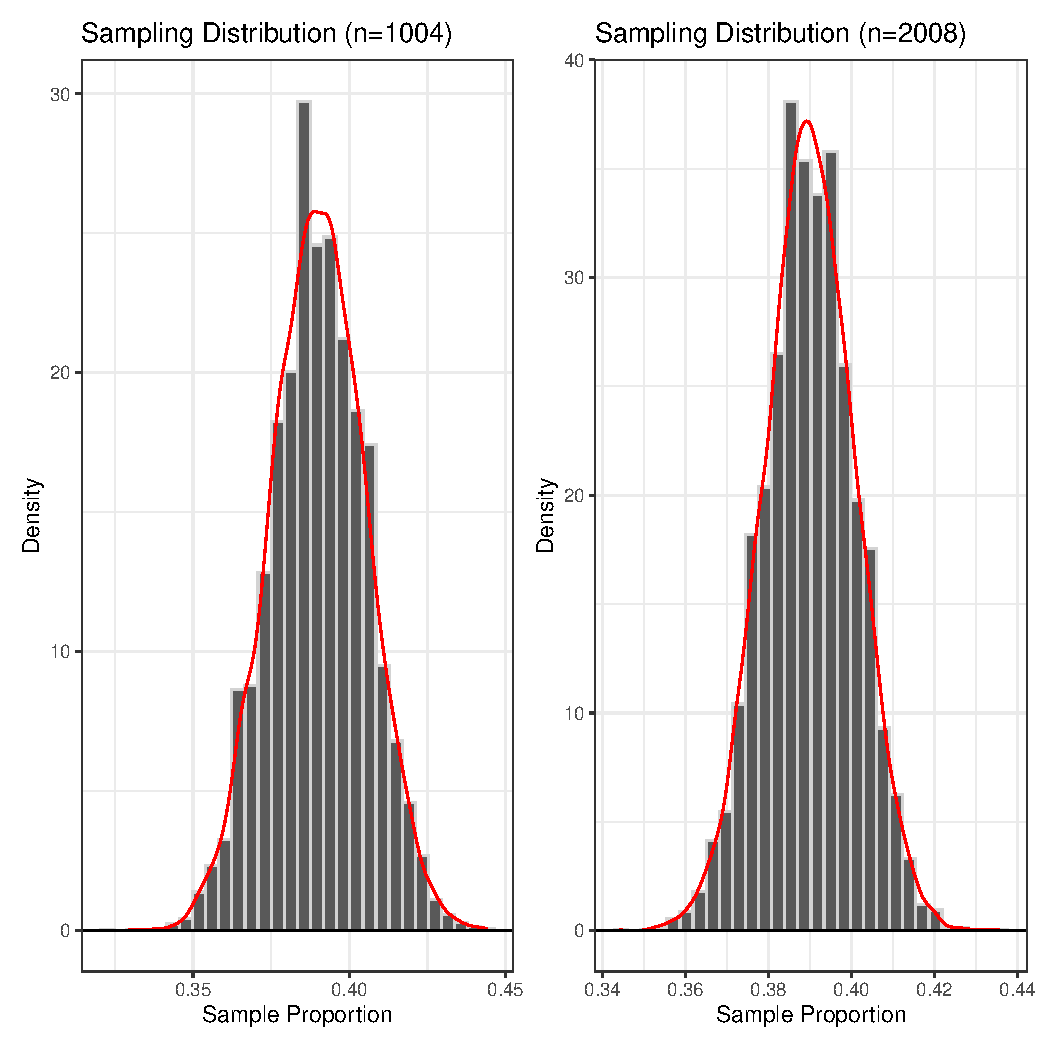
\includegraphics[width=\maxwidth]{figure/plot1-1} 
\end{knitrout}
\begin{figure}[H]
\begin{center}

\caption{Simulations for $n=1004$ and $n=2008$}
\label{simulationplot} %we can now reference plot1
\end{center}
\end{figure}

\pagebreak
\subsection{Resampling}
\begin{knitrout}\scriptsize
\definecolor{shadecolor}{rgb}{0.969, 0.969, 0.969}\color{fgcolor}
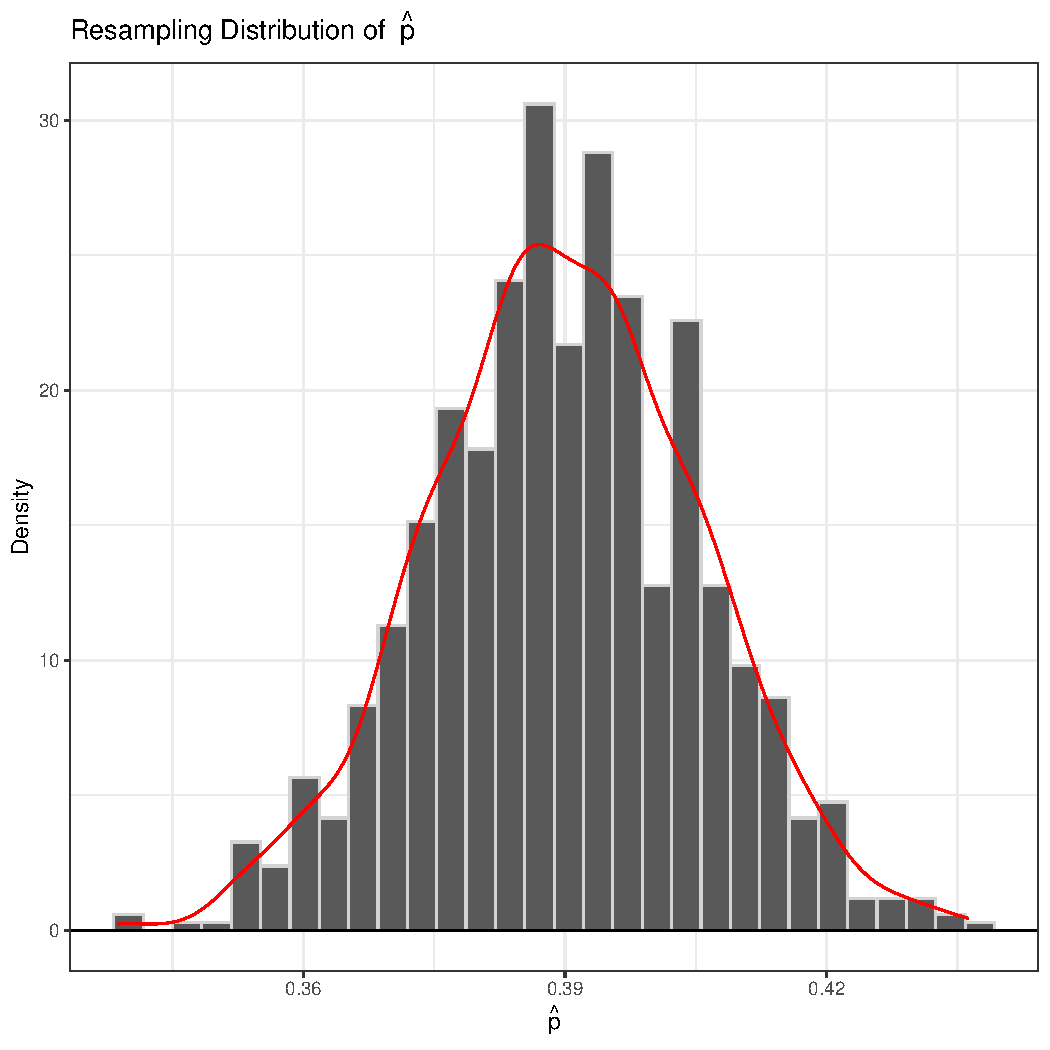
\includegraphics[width=\maxwidth]{figure/plot2-1} 
\end{knitrout}
\begin{figure}[H]
\begin{center}

\caption{Resampling Distribution of $\hat{p}$}
\label{resamplingplot} %we can now reference plot1
\end{center}
\end{figure}

\pagebreak
\subsection{Simulated Margin of Error}
\begin{knitrout}\scriptsize
\definecolor{shadecolor}{rgb}{0.969, 0.969, 0.969}\color{fgcolor}
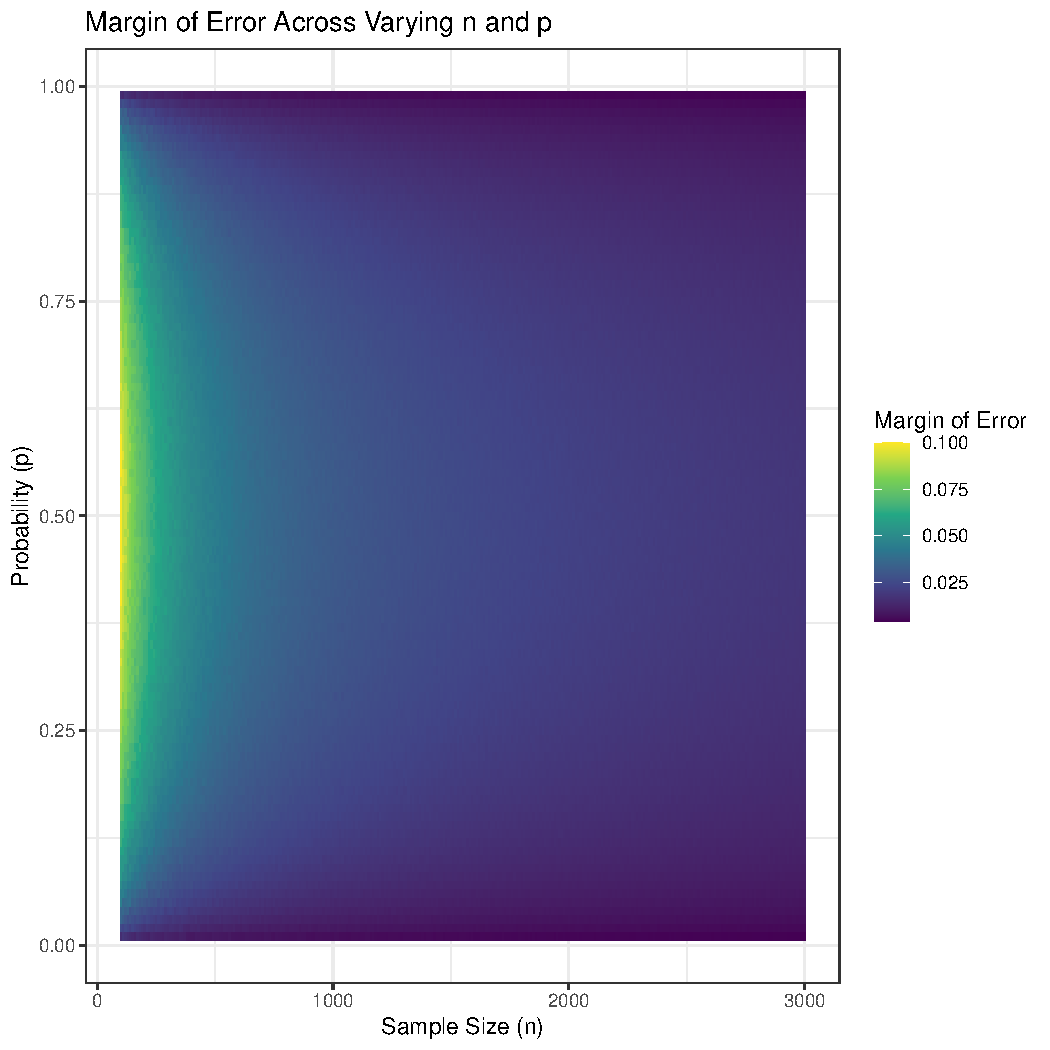
\includegraphics[width=\maxwidth]{figure/plot3-1} 
\end{knitrout}

\begin{figure}[H]
\begin{center}

\caption{Margin of Error Across $n$ and $p$}
\label{moeovernandp} %we can now reference plot1
\end{center}
\end{figure}

\pagebreak
\subsection{Wilson Margin of Error}
\begin{knitrout}\scriptsize
\definecolor{shadecolor}{rgb}{0.969, 0.969, 0.969}\color{fgcolor}
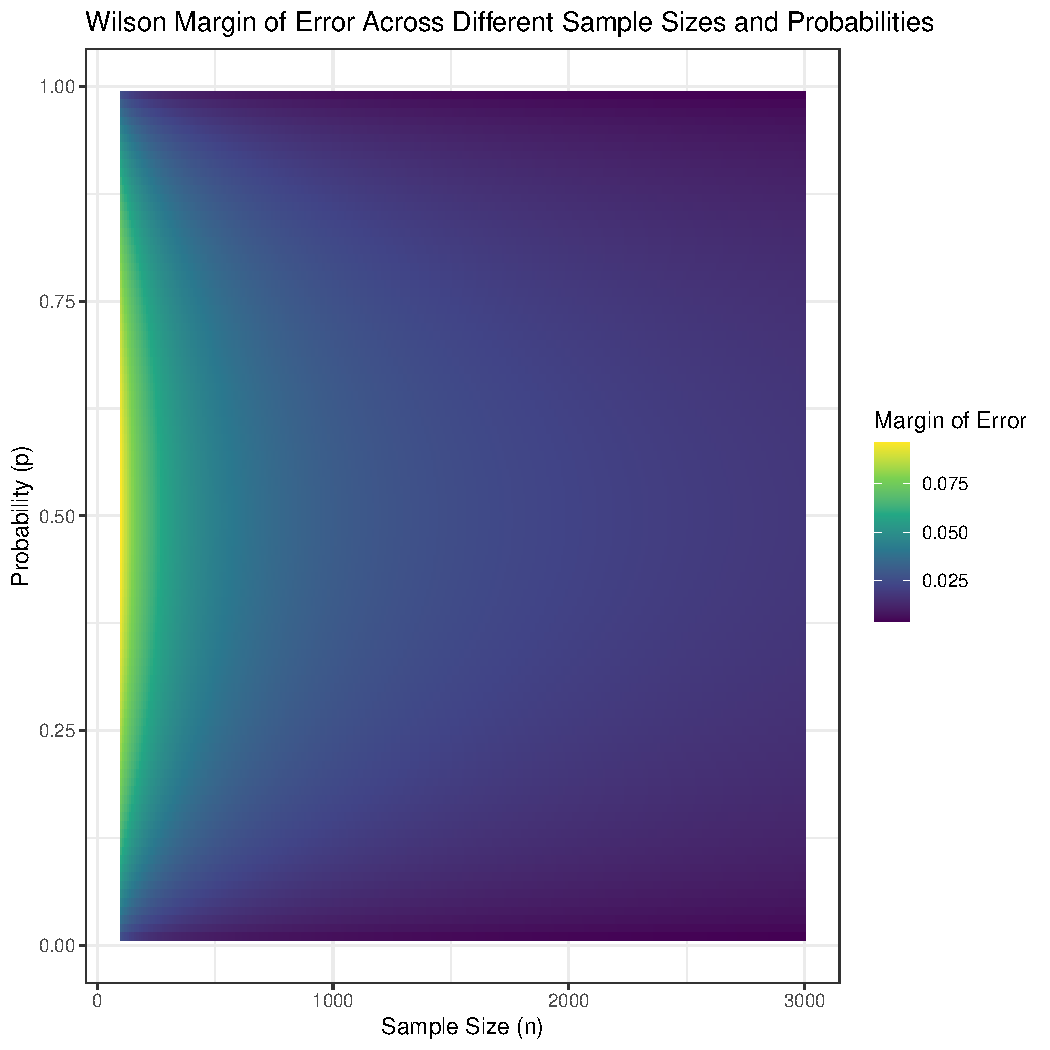
\includegraphics[width=\maxwidth]{figure/plot4-1} 
\end{knitrout}

\begin{figure}[H]
\begin{center}

\caption{Wilson Margin of Error}
\label{wilson} %we can now reference plot1
\end{center}
\end{figure}


\end{document}
